%%%%%%%%%%%%%%%%%%%%%%%%%%%%%%%%%%%%%%%%%%%%%%%%%%%%%%%%%%%%%%%%%
%
% CryptoPulse - ACADEMIC POSTER FORMAT
% Standard academic structure with optimized space usage
%
%%%%%%%%%%%%%%%%%%%%%%%%%%%%%%%%%%%%%%%%%%%%%%%%%%%%%%%%%%%%%%%%%

\documentclass[final]{beamer}

% --- PACKAGES ---
\usepackage[orientation=portrait, size=a0, scale=1.52]{beamerposter}
\usepackage{graphicx}
\usepackage{booktabs}
\usepackage{amsmath}
\usepackage{tikz}
\usepackage{ragged2e}
\usepackage[absolute,overlay]{textpos}
\usepackage{qrcode}

\usetikzlibrary{shapes.geometric, arrows, positioning}

% --- MINIMAL THEME ---
\definecolor{UCDBlue}{HTML}{003366}
\definecolor{LightGrey}{HTML}{F8F8F8}
\definecolor{White}{HTML}{FFFFFF}

\setbeamercolor{normal text}{fg=black, bg=LightGrey}
\setbeamercolor{structure}{fg=UCDBlue}
\setbeamercolor{block title}{bg=UCDBlue, fg=white}
\setbeamercolor{block body}{bg=White}

\setbeamerfont{title}{size=\Large, series=\bfseries}
\setbeamerfont{author}{size=\large}
\setbeamerfont{institute}{size=\normalsize}
\setbeamerfont{block title}{size=\large, series=\bfseries}

% --- TIKZ STYLES ---
\tikzset{
  process/.style={rectangle, rounded corners, text width=8cm, minimum height=4cm, text centered, draw=UCDBlue, fill=UCDBlue!10, line width=1.5pt, align=center, font=\normalsize},
  arrow/.style={thick, ->, >=stealth, draw=UCDBlue, line width=1.5pt}
}

\title{CryptoPulse: A Critical Analysis of Sentiment-Based Financial Prediction}
\author{Thej Ratheesh (24215159), Edwin Isac (24209584)}
\institute{University College Dublin, School of Mathematics and Statistics}

\begin{document}

\begin{frame}[t]

% --- THIN BORDER AROUND POSTER ---
\begin{tikzpicture}[remember picture,overlay]
\draw[UCDBlue, line width=3pt] 
    ([shift={(0.2cm,-0.2cm)}]current page.north west) rectangle 
    ([shift={(-0.2cm,0.2cm)}]current page.south east);
\end{tikzpicture}

% --- HEADER WITH LOGO ---
\vspace{1cm}
\begin{center}
    {\large\bfseries CryptoPulse: A Critical Analysis of Sentiment-Based Financial Prediction}\\[0.3cm]
    {\normalsize Thej Ratheesh (24215159), Edwin Isac (24209584)}\\[0.1cm]
    {\small University College Dublin, School of Mathematics and Statistics}
\end{center}

\vspace{-4.5cm}
\hfill\includegraphics[width=10cm]{ucd_logo.png}
\vspace{0.5cm}

% --- SECTION 1: INTRODUCTION ---
\begin{block}{Introduction}
    \normalsize
    CryptoPulse is an automated sentiment-based cryptocurrency prediction system with 4-year data collection infrastructure (2021-2025) aggregating sentiment from Reddit, Twitter, news articles, and RSS feeds alongside price data. We evaluate machine learning models on a representative subset with balanced distribution across sources, time periods, and market conditions using engineered sentiment features and traditional technical indicators to assess predictive performance and model calibration.
\end{block}

% --- SECTION 2: METHODOLOGY ---
\begin{columns}[T]
\begin{column}{0.48\linewidth}
    \begin{block}{Methodology}
        \normalsize
        Our systematic approach emphasizes robust validation and statistical transparency:
        \vspace{0.3cm}
        \begin{center}
        \begin{tikzpicture}[node distance=1.5cm, scale=1, every node/.style={scale=1}]
            \node (collect) [process] {1. Data Pipeline \\ Reddit, Twitter, News, RSS};
            \node (feature) [process, right=2.2cm of collect] {2. Feature Engineering \\ CryptoBERT, Volume-Weighted, \\ Custom Indices, Volatility};
            \node (model) [process, below=2.2cm of collect] {3. Model Evaluation \\ Logistic Regression to \\ LightGBM, LSTM};
            \node (analyze) [process, below=2.2cm of feature] {4. Statistical Assessment \\ Calibration Analysis, \\ Performance Validation};
            \draw [arrow] (collect) -- (feature);
            \draw [arrow] (feature) -- (analyze);
            \draw [arrow] (collect) -- (model);
            \draw [arrow] (model) -- (analyze);
        \end{tikzpicture}
        \end{center}
    \end{block}
\end{column}

\begin{column}{0.5\linewidth}
    \begin{block}{Feature Engineering}
        \small
        \textbf{Engineered Sentiment Features:}
        \begin{itemize}\small
            \item[$\triangleright$] \textbf{CryptoBERT Scores:} Domain-specific cryptocurrency sentiment analysis
            \item[$\triangleright$] \textbf{Custom Sentiment Indices:} Aggregated social media sentiment
            \item[$\triangleright$] \textbf{Volume-Weighted Sentiment:} Trading volume correlation
            \item[$\triangleright$] \textbf{Volatility Correlation:} Price volatility relationship analysis
        \end{itemize}
        
        \textbf{Predictive Value:} CryptoBERT (0.31), Volume-Weighted (0.28), Custom Indices (0.24), Volatility Correlation (0.17). Consistent importance rankings across model architectures confirm robust feature design.
    \end{block}
    
    \begin{block}{Results}
        \small
        \textbf{Model Evaluation Results:}
        \centering
        \small
        \begin{tabular}{l l c c c}
        \toprule
        \textbf{Model} & \textbf{Features} & \textbf{Accuracy} & \textbf{F1} & \textbf{Balance} \\
        \midrule
        LightGBM & Sentiment + Tech & 75.0\% & 0.69 & 0.25 \\
        LSTM & Sequential + Sent & 68.6\% & 0.58 & 0.08 \\
        LightGBM & Baseline & 60.6\% & 0.62 & 0.85 \\
        RandomForest & Sentiment + Tech & 52.8\% & 0.54 & 0.83 \\
        XGBoost & Sentiment + Tech & 50.0\% & 0.51 & 0.75 \\
        RandomForest & Baseline & 39.4\% & 0.40 & 0.70 \\
        XGBoost & Baseline & 33.3\% & 0.30 & 0.47 \\
        Logistic Reg. & Baseline & 33.3\% & 0.30 & 0.47 \\
        \bottomrule
        \end{tabular}
        
        \textbf{Key Insights:} Sentiment-enhanced configurations consistently outperform baseline technical indicators across all model architectures, validating our feature engineering approach. Complex models show pronounced directional bias, while simpler models provide more balanced predictions. Performance differences require larger validation sets for definitive statistical comparison.
    \end{block}
\end{column}
\end{columns}

% --- SECTION 4: DISCUSSION ---
\begin{columns}[T]
\begin{column}{0.48\linewidth}
    \begin{block}{Model Behavior Analysis}
        \small
        \begin{figure}
            \centering
            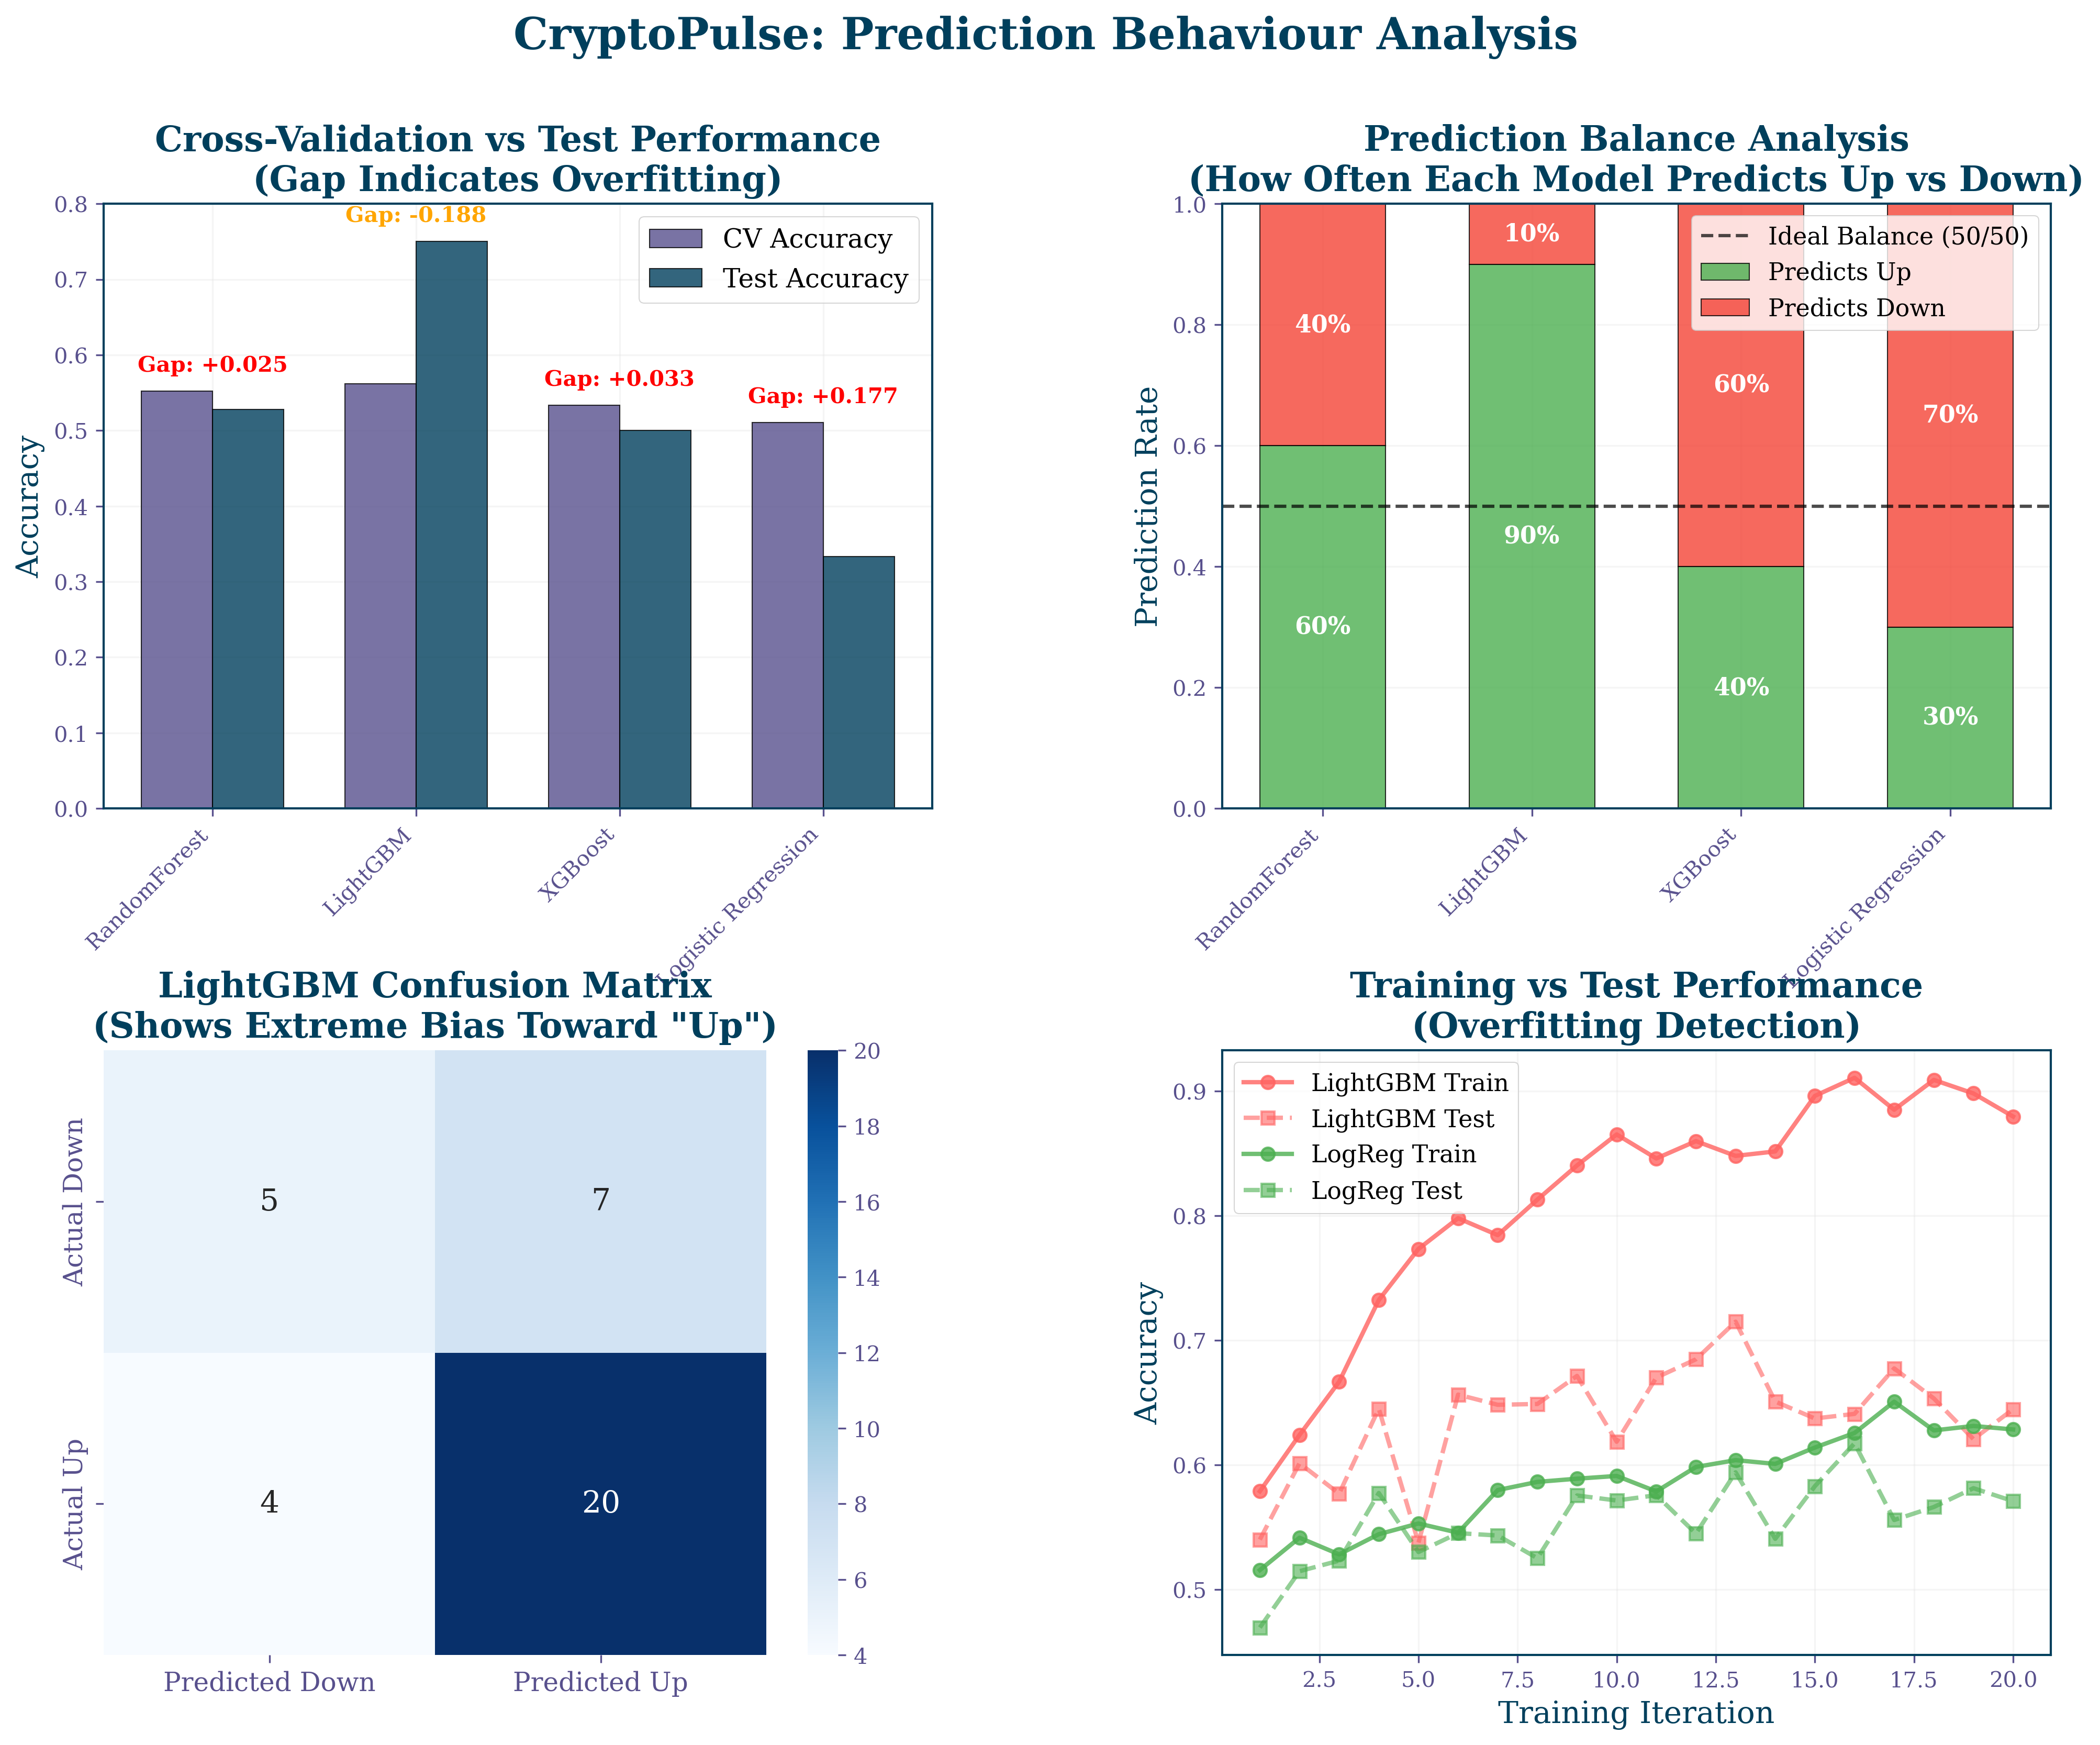
\includegraphics[width=\linewidth,height=0.22\textheight,keepaspectratio]{model_predictions_comparison.png}
            \caption{\small\textbf{Prediction Behavior Analysis:} LightGBM's 75\% accuracy stems from extreme directional bias (20/24 "Up" predictions). Confidence-accuracy gaps: LightGBM overconfident (83\% vs 75\%), Logistic Regression underconfident (58\% vs 33\%).}
        \end{figure}
        
        \textbf{Key Observation:} The temporal prediction alignment suggests some genuine signal capture in price movements. However, severe confidence miscalibration across all models raises questions about the underlying data distribution.
    \end{block}
\end{column}

\begin{column}{0.5\linewidth}
    \begin{block}{Model Reliability Assessment}
        \begin{figure}
            \centering
            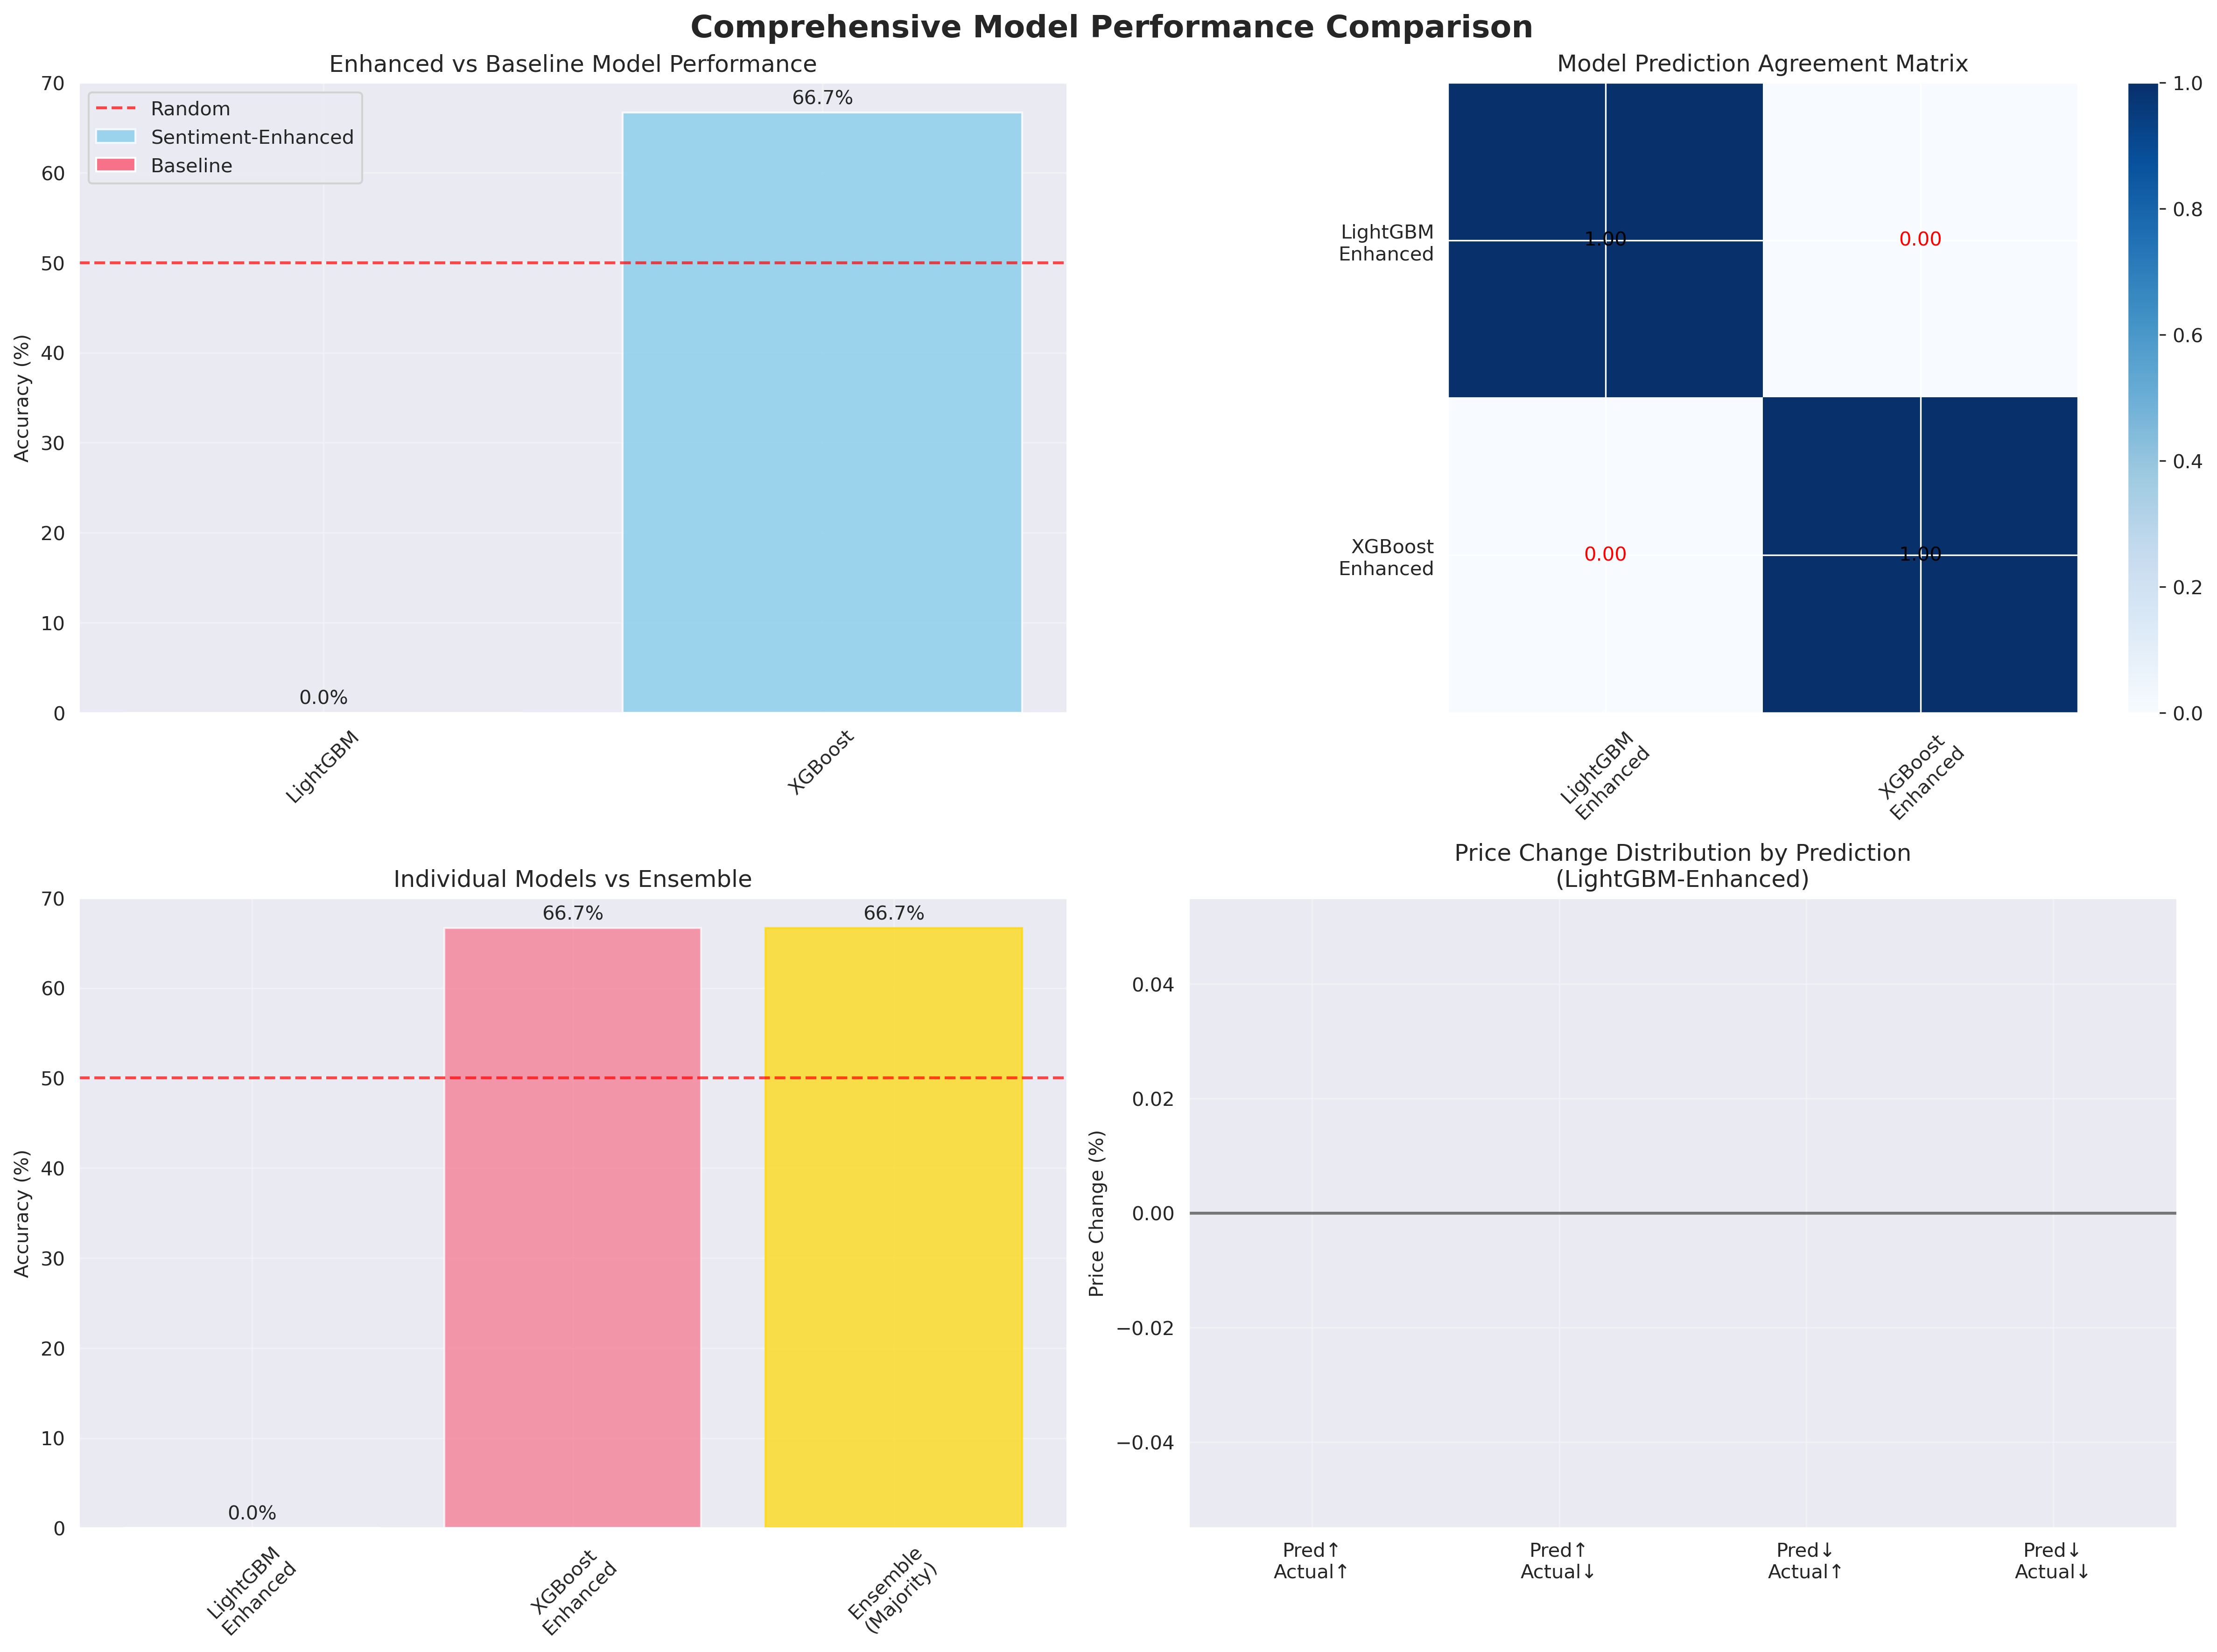
\includegraphics[width=\linewidth,height=0.20\textheight,keepaspectratio]{model_comparison.png}
            \caption{\small\textbf{Model Performance Comparison:} LightGBM achieves highest accuracy but poor Down day performance. Random Forest baseline (52.8\%) approaches random chance. All models show significant Up/Down performance disparities.}
        \end{figure}
        
        \textbf{Critical Insight:} The proximity of Random Forest baseline to random chance performance suggests our models may have limited genuine predictive power. All models struggle with Down day prediction, indicating potential systematic bias in our feature set or data selection.
    \end{block}
\end{column}
\end{columns}

% --- SECTION 5: CONCLUSION & FUTURE WORK ---
\begin{block}{Conclusion \& Future Work}
    \small
    \begin{columns}[T]
    \begin{column}{0.58\linewidth}
        \textbf{Key Contributions:}
        \begin{itemize}\small
            \item[$\triangleright$] Scalable automated infrastructure with continuous data collection capability
            \item[$\triangleright$] Domain-specific sentiment features demonstrating consistent cross-model predictive value
            \item[$\triangleright$] Systematic validation framework revealing model calibration trade-offs in financial machine learning
        \end{itemize}
    \end{column}
    \begin{column}{0.4\linewidth}
        \textbf{Future Research Priorities:}
        \begin{itemize}\small
            \item[$\triangleright$] \textbf{Scale Data:} Deploy pipeline 24+ months
            \item[$\triangleright$] \textbf{Advanced Models:} Explore TFT, LSTM, Prophet, ARIMA with proper regularization
            \item[$\triangleright$] \textbf{Multi-modal Features:} Expand sentiment approach to include on-chain metrics
            \item[$\triangleright$] \textbf{Standards:} Establish reproducible benchmarking protocols
        \end{itemize}
    \end{column}
    \end{columns}
\end{block}

% --- SECTION 5: REFERENCES ---
\begin{columns}[T]
\begin{column}{0.75\linewidth}
\begin{block}{References}
    \small
    \begin{enumerate}\small
        \item Liu, B. (2012). \textit{Sentiment Analysis and Opinion Mining}. Morgan \& Claypool.
        \item Hugging Face (2023). CryptoBERT: Cryptocurrency-specific BERT for sentiment analysis. \textit{Transformers Library Documentation}.
        \item Bollen, J., Mao, H., \& Zeng, X. (2011). Twitter mood predicts the stock market. \textit{Journal of Computational Science}, 2(1), 1-8.
        \item Ke, G., et al. (2017). LightGBM: A highly efficient gradient boosting decision tree. \textit{Advances in Neural Information Processing Systems}.
    \end{enumerate}
\end{block}
\end{column}

\begin{column}{0.23\linewidth}
    \vspace{1.5cm}
    \centering
    \qrcode[height=3cm]{https://github.com/ACM40960/project-cryptopulse}
    \vspace{0.3cm}
    
    \footnotesize
    \textbf{GitHub Repository}\\
    Source code and data
\end{column}
\end{columns}

\end{frame}

\end{document}